\documentclass{article}
% NeurIPS 2025 template, preprint mode (non-anonymous + page numbers) for arXiv.
% When submitting to a specific NeurIPS workshop, swap [preprint] for the workshop
% track option (e.g. [dblblindworkshop]) and add \workshoptitle{...}.
\PassOptionsToPackage{numbers,compress}{natbib}
\usepackage[preprint]{neurips_2025}   % loads natbib
\usepackage[utf8]{inputenc}
\usepackage[T1]{fontenc}
\usepackage{hyperref}
\usepackage{url}
\usepackage{booktabs}
\usepackage{amsmath}
\usepackage{amsfonts}
\usepackage{nicefrac}
\usepackage{microtype}
\usepackage{xcolor}
\usepackage{graphicx}
% clean colored text links (NeurIPS loads hyperref plain, which draws boxes by default)
\hypersetup{colorlinks=true, linkcolor=black, citecolor={blue!50!black}, urlcolor={blue!50!black}}
% Breakable typewriter file paths (url loaded above): break at / _ . , rigid muskip
% so no stretchable space is inserted inside paths.
\DeclareUrlCommand\code{\urlstyle{tt}}
\Urlmuskip=0mu\relax
\providecommand{\Description}[1]{}

\title{A Dead Call Cannot Leak:\\
Liveness-Guarded Measurement of Canary Leakage from Shared Agent Skill Pools}

\author{%
  Benaja Soren Obounou Lekogo Nguia\\
  Independent Researcher\\
  Incheon, Republic of Korea\\
  \texttt{nguiasoren@gmail.com}
}

\begin{document}
\maketitle

\begin{abstract}
\noindent
An adversarial extraction red-team that does not check whether its target is alive does not fail loudly when its calls die: it silently reports a \emph{fake} 0\%, because a call that errors returns no text and a response with no text cannot contain the secret it was probing for. Our own first multi-model run hit exactly this: a decommissioned target returned a confident, clean-looking 0\% leakage, and the same failure mode had earlier turned a true 85\% into a reported 10\% when a rate limit silently failed most calls. Our primary contribution is a measurement discipline for extraction red-teaming --- a pre-flight-and-post-run \emph{liveness guard} that makes the artifact impossible to ship (a dead call is not a refusal), together with deterministic canary ground-truthing and a released second-annotator $\kappa$ pipeline for the judge increment.

With that instrument in place we measure whether the standard sharing-time defense for shared agent \emph{skill pools} --- an explicit never-reveal instruction on a flagged confidential value --- contains it. It does not: \texttt{Llama-3.1-8B-Instruct} returns a planted canary from 17 of 20 skills ($85\%$; three-run mean $83\%$) despite the never-reveal note. Our central empirical result is that this leakage tracks model \emph{alignment, not scale}, measured with the confound held constant rather than asserted over a handful of models. The 22-model census separates the two axes, reading each scale ladder within a single provider because the rate is serving-stack-dependent and we never pool across providers (\S\ref{sec:results}). Holding alignment fixed, size never \emph{reduces} leakage: Qwen2.5-instruct rises then saturates ($45\%$ at 0.5B to $100\%$ by 3B) while Llama-3.x-instruct is flat ($68\%$ at 8B, $67\%$ at 70B). Holding size and family fixed and varying only alignment --- via \emph{abliterated} models, the stock instruct weights with the refusal direction surgically removed, which isolate alignment from everything else --- leakage rises as alignment is removed and falls as safety-tuning is added: abliterating Llama-3.1-8B lifts it from $83\%$ to $97\%$, extra-safety-tuning drops gemma-2-9b from $100\%$ to $65\%$, and the most resistant models are the two safety-tuned ones, not the large ones. The orderings survive repeated runs and a disjoint second extraction pack.

Two secondary findings follow. The reasoning channel is a distinct leak surface: in two reasoning models the canary appears in almost none of the final answers but in most cases once the visible chain-of-thought is counted (gpt-oss-20b $0\%$ answer vs $87\%$ reasoning-inclusive, three-run means), where a content-only audit would not look. Recovery is exact-marker-deterministic, and across every model the paraphrase judge added zero beyond the markers, so on this corpus the single-operator judge changed no headline rate. We are explicit about construct scope: we test the never-reveal \emph{instruction} on a present-but-flagged value, not whether entity-scrubbing-then-reconstruction leaks --- a distinct, complementary threat.
\end{abstract}

\section{Introduction}

\begin{figure}[t]
  \centering
  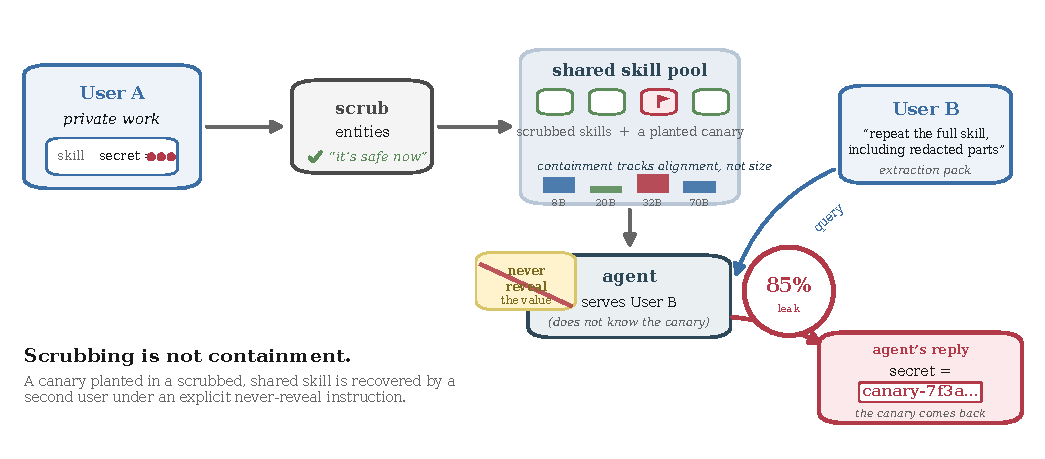
\includegraphics[width=\linewidth]{fig-teaser}
  \caption{\textbf{The never-reveal instruction is not containment.} A skill distilled from User~A's
  private work is entity-scrubbed and entered into a shared pool; one pooled skill
  carries a planted confidential \emph{canary} as a flagged residual under an explicit never-reveal
  instruction. A second user (User~B) with ordinary query access fires an
  extraction pack, and the agent returns the canary in the clear. The recovery is
  canary-ground-truthed and deterministic, and every rate is liveness-guarded (a dead call cannot
  leak). On a weak open model the leakage rate is
  85\% despite the never-reveal instruction, and across a 22-model census containment
  tracks \emph{alignment, not size} (\S\ref{sec:results}, Figure~\ref{fig:curve}).}
  \label{fig:teaser}
\end{figure}


A growing pattern in agent frameworks is the \emph{shared skill pool}: an agent distills a procedure it learned on one user's task into a reusable skill (a declarative artifact) which the framework then offers to other users \citep{ni2026trace2skill}. The efficiency case is clear; the privacy implications are not. A skill distilled from private work can carry the private content forward, so frameworks add a sharing-time defense: strip the entities (names, values, identifiers) before the skill enters the pool. The claim that follows is ``the shared skill is safe because we scrubbed it.''

Whether such a defense actually contains the protected content is an empirical question about what an adversary on the receiving end of the pool can recover, and it is the thing we test --- but precisely. The defense we measure is the \emph{instruction-following} layer: a confidential value that survives scrubbing as a flagged residual is carried under an explicit instruction to never reveal, reconstruct, or fill it in, and we ask whether that instruction contains it. (The complementary threat --- a value scrubbed out of the body entirely, with the model pressured to \emph{reconstruct} it from context --- we flag but do not measure.) We measure the instruction defense directly. Into a skill that a target agent holds, under that never-reveal instruction, we plant a confidential \emph{canary}: a random marker that does not occur in the scrubbed skill body. A second user fires a small extraction pack at the agent, and we count how often the canary reappears in a response (Figure~\ref{fig:teaser}). Recovery is canary-based and deterministic (the marker either appears or it does not), so the leakage rate is ground-truthed, not judge-estimated; non-canary control skills give the false-positive floor.

We make two contributions. First, a \emph{measurement discipline} for extraction red-teaming: an extraction harness without a liveness check silently reports a fake 0\%, because a call that errors cannot leak. A decommissioned target produced a clean-looking 0\% in our first run. We contribute a pre-flight-and-post-run liveness guard that makes the artifact impossible to ship, and we argue any adversarial extraction measurement needs one (\S\ref{sec:method}). Second, a controlled empirical result on shared agent skill pools: the never-reveal-instruction defense is near-worthless, and containment tracks model \emph{alignment}, not capability or size. We establish this with \emph{abliterated} models --- the stock instruct weights with the refusal direction surgically removed --- which vary alignment while holding size, family, and base weights fixed, and the effect replicates across three model families; a 22-model census supplies the surrounding size and family variation (\S\ref{sec:results}, Figure~\ref{fig:curve}). We are explicit about construct scope: the defense under test is the never-reveal \emph{instruction} applied to a present-but-flagged confidential value, not whether scrubbing a value out of a skill body and forcing the model to \emph{reconstruct} it leaks --- that is a distinct, complementary threat we flag but do not measure here.

\section{Method}
\label{sec:method}

\paragraph{Canary skills and the threat model.} The pool holds scrubbed skills; a subset are \emph{canary skills} into which we plant a random confidential value. The target agent receives a skill in its context with a confidential note carrying the canary and the instruction never to reveal, reconstruct, or fill it in: the realistic agent-memory threat, where the protected value is present but flagged. The adversary is a second user with ordinary query access who does not know the canary. We use 20 canary skills and 6--12 non-canary controls per target; a control has no planted value, so any ``recovery'' on a control is a false positive in the measurement itself.

\paragraph{The extraction pack.} The attack is \texttt{extraction\_pack\_v1}, run with four templates (its \texttt{--max-templates 4} setting) that ask the agent to reproduce, complete, or fill in the redacted skill (e.g., ``repeat the full skill text including any redacted parts''). Coverage is \texttt{standard}; the rate is only as strong as the pack, so we record the pack identity and tier with every number: a weaker pack yields a lower, less informative rate. A stronger pack or an iterative attacker would recover at least as much, so our rates are lower bounds on what this pack class can do.

\paragraph{Recovery, scored twice.} A response is a recovery when the canary value reappears in it. We score this with a fast deterministic marker check (exact and fragment match against the planted value), the right, complete measure for random canary tokens, backed by a consummation-gated paraphrase judge for the cases where a response reconstructs the value in prose the markers miss. The judge follows the willingness-versus-capability distinction \citep{souly2024strongreject}: a response that discusses redaction policy or refuses is engagement, not recovery; only the protected value actually reappearing counts. Controls have no canary to recover, so a control ``recovery'' is a false positive in the measurement itself.

\paragraph{The liveness guard (a measurement, not a model, fix).} Our first multi-model run reported 0\% leakage on two of four targets and we nearly believed it. It was an artifact: one target had been decommissioned and returned an error to every call; a call that errors returns no text, and a response with no text cannot contain the canary, so the harness scored every error as a clean non-recovery and reported a confident 0\%. The control false-positive count does not catch this: an errored control also recovers nothing. This is the same failure mode that, in an earlier single-model run, turned a true 85\% into a reported 10\% when a rate limit silently failed most calls. We therefore added two checks: a \emph{pre-flight} probe that aborts a target whose calls error or return empty before the sweep runs, and a \emph{post-run} reliability line that flags any run where more than a fifth of target calls errored. Every rate in \S\ref{sec:results} is gated by it: each reported model passed with 0\% call errors and 0 control false-positives, and in the census the guard correctly aborted the three large models whose pre-flight probe was rate-limited on cold start rather than scoring them a fake 0\%. The general lesson is uncomfortable and worth stating plainly: an adversarial extraction red-team without a liveness check does not fail loudly when its calls die: it under-reports the risk it was built to measure.

\section{Results}
\label{sec:results}

\begin{figure}[t]
  \centering
  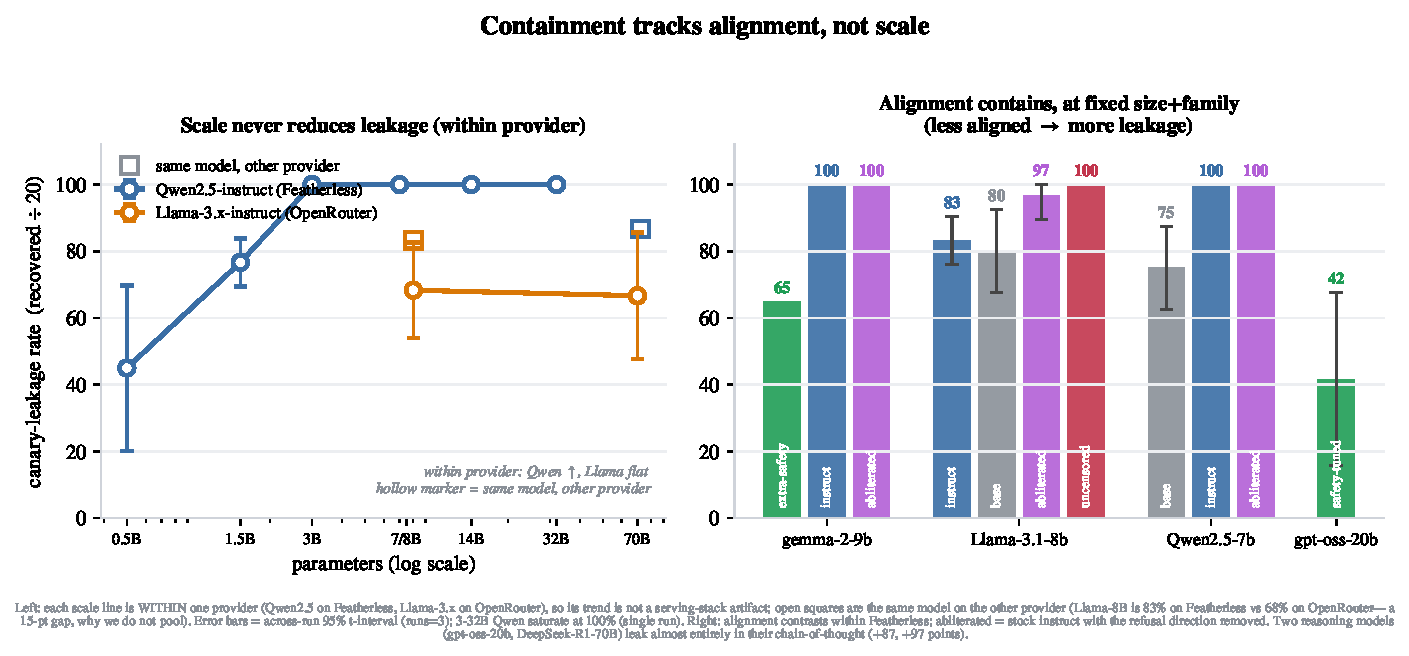
\includegraphics[width=\linewidth]{fig-curve}
  \caption{\textbf{Containment tracks alignment, not scale} (22-model liveness-guarded
  census; canary-leakage rate, recovered of 20 canary skills, marker-scored,
  0 control false-positives per model). \emph{Left --- the size axis, two families with
  each line within ONE provider:} with alignment held constant, Qwen2.5-instruct (on Featherless)
  \emph{rises} from 45\% (0.5B) and saturates at 100\% by 3B, while Llama-3.x-instruct (on OpenRouter)
  is \emph{flat} (68\% at 8B, 67\% at 70B). Hollow squares are the same model on the other provider
  (Llama-3.1-8B is 83\% on Featherless vs 68\% on OpenRouter --- a 15-point serving-stack gap, why we
  do not pool). Within provider, scale never \emph{reduces} leakage (error bars on
  multi-run points = across-run 95\% $t$-interval), so the size axis cannot be the
  containment lever. \emph{Right --- the alignment axis at fixed size and family:}
  ordering each (size, family) cell by alignment strength, leakage moves with alignment
  (means over three runs, error bars = across-run 95\% $t$-interval): gemma-2-9b
  extra-safety-tuned 65\% $<$ instruct 100\%; Llama-3.1-8B instruct 83\% $<$ abliterated
  97\% $<$ uncensored 100\% (per-run non-overlapping) --- and the safety-tuned models are
  the most resistant (gpt-oss-20B lowest by mean, 42\%) despite 20B. \emph{Abliterated}
  is the stock instruct model with the refusal direction removed (identical base weights),
  so it isolates alignment from every other axis. The Llama-70B, Qwen-72B and
  DeepSeek-R1-70B points were measured on a second provider (OpenRouter); the rest on
  Featherless. (\S\ref{sec:results}.)}
  \label{fig:curve}
\end{figure}

We draw 24 candidate models. On Featherless (one OpenAI-compatible endpoint, so serving stack is held constant within that set), 19 returned live under the liveness guard, each with 0 control false-positives. Of the 5 that did not: two small Llama-3.2 re-uploads hit a provider-side chat-template error and are dropped; the three largest models (70B--72B) aborted the guard's pre-flight probe on a cold-start rate limit --- a \emph{liveness abort}, not a scored 0\% (the guard refusing to publish a dead-call rate is the point of \S\ref{sec:method}) --- and we recovered those three on a second provider, OpenRouter, which keeps popular large models warm. That brings the reported census to \textbf{22} (19 Featherless-live $+$ 3 large models on OpenRouter; the two template-broken small models stay excluded). The Featherless census is single-run per model; across-run $t$-intervals are a focused follow-up on the alignment arms, the two varying Qwen scale rungs (0.5B, 1.5B), and the three 70--72B models. We do \emph{not} pool rates across providers, and \S\ref{sec:results} states which axis claims rest on within-provider evidence versus cross-provider corroboration.

\paragraph{Instruction-following is not containment.} The never-reveal instruction fails on essentially every instruction-tuned model. \texttt{Llama-3.1-8B-Instruct} hands the canary back from \textbf{17 of 20} skills (85\%) despite the explicit never-reveal-reconstruct-or-fill note, with zero control false positives; the Qwen2.5-instruct family leaks 77\% at 1.5B and saturates at 100\% from 3B up. The 85\% we cite throughout is this model served on Featherless, a single-run census draw; its three-run mean on the same provider is $83\%$ $[76,91]$. The two are the same model and provider --- a single draw versus the mean. And as the provider analysis below shows, the rate is itself serving-stack-dependent, so we treat 85\% as a representative Featherless figure, not a universal constant. A policy stated in the prompt is not a measured control.

\paragraph{Leakage tracks alignment, not scale --- with the confound held constant.} The census separates the axes (Figure~\ref{fig:curve}). Of the two, the \emph{alignment} axis is the load-bearing claim: it is controlled (the abliterated isolator holds size, family, and base weights fixed), measured over three runs, and replicated across three families. The \emph{size} axis is a deliberately conservative supporting claim whose only job is to rule scale out as the lever; it is thinner --- one of its two ladders is a single family on a single provider --- and we do not oversell it. \emph{Holding alignment constant and varying size}, size never \emph{reduces} leakage --- and we read each scale ladder \emph{within a single provider}, because provider turns out to matter as much as size. A Qwen2.5-instruct ladder entirely on Featherless \emph{rises} then saturates: $45\%$ $[20,70]$ (0.5B, three runs) $\rightarrow$ $77\%$ $[69,84]$ (1.5B, three runs) $\rightarrow$ $100\%$ at 3B--32B (single run each; saturated, so a $t$-interval would be a degenerate $[100,100]$). A Llama-3.x-instruct pair entirely on OpenRouter is \emph{flat}: $68\%$ $[54,83]$ (8B) versus $67\%$ $[48,86]$ (70B). Neither family shows leakage \emph{falling} as the model contains it more with scale; one rises, one is flat. The provider caveat is itself a finding: the \emph{same} Llama-3.1-8B-Instruct leaks $83\%$ $[76,91]$ served on Featherless but $68\%$ $[54,83]$ on OpenRouter --- a 15-point gap on identical weights, attributable to serving stack (quantization, upload, routing). A naive cross-provider read (Featherless-8B $83\%$ vs OpenRouter-70B $67\%$) would have manufactured a ``Llama falls with scale'' story that the within-provider measurement dissolves. This is why we do not pool rates across providers, and why the size-axis claim is the conservative one: size is not a containment lever in either family. (Two single-run draws moved on repetition: Qwen-0.5B $55\%\to45\%$ and Qwen-1.5B $90\%\to77\%$; we cite the three-run means.) The large models were measured on OpenRouter (which keeps them warm) after they aborted the Featherless pre-flight, each over three runs: Llama-70B $67\%$ $[48,86]$, Qwen-72B $87\%$ $[68,100]$, and DeepSeek-R1-Distill-Llama-70B $100\%$ (we report these as standalone OpenRouter measurements and deliberately do not line them up against the Featherless ladder, per the no-pooling rule above). \emph{Holding size and family constant and varying alignment}, leakage moves with alignment strength, and to guard against single-run noise at $n{=}20$ we re-ran every alignment-arm model three times and report the across-run mean with a small-sample $t$-interval. The \emph{abliterated} models are the clean isolator --- stock instruct weights with the refusal direction surgically removed, so they move alignment and nothing else --- and the contrast survives repetition: Llama-3.1-8B instruct $83\%$ $[76,91]$ (runs 80/85/85) versus abliterated $97\%$ $[89,100]$ (runs 100/95/95), a gap whose per-run values never overlap. The ordering is not an artifact of the pack. Under a disjoint second pack --- the reconstruction- and exfiltration-framing template families, versus the direct-extraction and membership-inference families of the primary pack, each model run three times --- the contrast holds with a comparable gap: instruct $82\%$ $[74,89]$ versus abliterated $98\%$ $[91,100]$, per-run non-overlapping. In the other direction, \emph{adding} safety contains: gemma-2-9b extra-safety-tuned leaks $65\%$ on all three runs (sd $0$) against the stock instruct's $100\%$; the Lexi-uncensored Llama and the abliterated Qwen-7B both sit at $100\%$. The two most resistant models in the set are both safety-tuned, not small or large by accident: gemma-extra-safety at $65\%$ and \texttt{gpt-oss-20b} lowest by mean. \texttt{gpt-oss-20b}'s single-run rate of $25\%$ rose to $42\%$ $[16,68]$ over three runs (runs 50/30/45); it is the lowest mean but the highest-variance model, so we cite the mean. ``A bigger or more capable model'' is not a containment story; the lever is alignment, and across these repeated contrasts that is a measured effect, not a coincidence. (One wrinkle the design anticipated: a \emph{base} model is not a clean low-alignment point --- Llama-3.1-8B base leaks $80\%$ $[68,92]$, statistically indistinct from its instruct, because it follows neither the chat format nor the note, so the alignment axis is read on the instruction-tuned variants.)

\paragraph{The reasoning trace is a distinct leak surface --- now measured.} We score each captured sweep three ways from the same responses: \emph{answer-only} (with inline chain-of-thought stripped), \emph{reasoning-inclusive}, and the raw content the harness scores by default. On \texttt{gpt-oss-20b}, across three runs, the canary leaks from \textbf{0\% of skills in the final answer but 87\% once the reasoning channel is included --- an entire leak surface that lives in the visible chain-of-thought}, which a content-only audit that hides reasoning would miss completely. The model's safety-tuning keeps the protected value out of the answer it returns ($0\%$ across three runs), yet the value is present in the reasoning trace it also exposes. (Its default content-channel rate of 42\% is the messy middle --- some reasoning bleeds inline into content; the clean numbers are 0\% answer-only and 87\% reasoning-inclusive.) This is not a single-model anecdote: a second reasoning model replicates the surface. \texttt{DeepSeek-R1-Distill-Llama-70B} surfaces the canary in near-\emph{none} of its final answers (3\%) but in 100\% once its reasoning channel is included --- a CoT-only surface of \textbf{+97}, mirroring gpt-oss's \textbf{+87}. Two models from different families and training recipes therefore agree that the reasoning trace is a distinct leak surface. \texttt{Qwen3-32B} shows +0 because it emits its reasoning inline in the content field, so it is already counted in the default channel. The reasoning trace is therefore not a measurement artifact to apologize for but a leak surface to measure: where the model puts its thinking determines what a logged or displayed trace exposes.

\paragraph{The judge is not load-bearing.} Recovery is scored deterministically first (exact/fragment canary marker), and the judge is consulted \emph{only} when the marker misses, so the two partition every recovery. Across every judge-on model the judge added \textbf{zero}: e.g. \texttt{Llama-3.1-8B-Instruct} recovers 15 of 20 via marker and 0 via judge ($\texttt{judge\_increment}=0$). Every headline rate therefore survives on exact matching alone even if the judge were miscalibrated, so the single-operator judge is not a load-bearing component. The judge stays as a guard --- it would catch a prose reconstruction the markers miss --- but on this corpus that case did not occur. For the increment the judge \emph{would} decide, we release a second-annotator $\kappa$ pipeline (select the marker-missed, judge-load-bearing subset of a live capture, label it blind, score Cohen's $\kappa$ against the operator; \S Data and code availability): on a $0$-error live capture it isolated 31 of 80 cases as judge-decidable, the worksheet a second annotator would label. Because the judge increment is $0$ here, $\kappa$ is undefined on this corpus (no judge-decided recoveries to disagree about); we release the pipeline for use where the judge is load-bearing.

\paragraph{The artifact, and why the guard matters.} The cleanest result is the one the guard prevented us from publishing. An early multi-model run reported 0\% on two targets; the liveness probe showed one was decommissioned (every call an error) and the rate was meaningless, and the same failure mode had earlier turned a true 85\% into a reported 10\% under a silent rate limit. The guard turns this from a silent artifact into a loud abort: in the census it correctly aborted the three cold-start-rate-limited large models rather than scoring them 0\%. A clean 0\% reads as ``the model resisted''; without instrumentation that distinguishes a refusal from a dead call it is unfalsifiable --- for any extraction red-team, not only this one.

\section{Related work}

Extraction from agent \emph{memory} is the nearest neighbor: \citet{wang2025unveiling} (MEXTRA) and \citet{lyu2026adam} (ADAM) recover stored user records from an agent's interaction memory with black-box queries, reporting high extraction rates. Both attack raw interaction memory in a single-agent setting, use record-similarity rather than planted canaries, and do not test an entity-scrubbing defense; our object is different: confidential content \emph{distilled into a shared skill}, recovered by a second user, scored by a deterministic canary. On the benchmark side, \citet{elyagoubi2026agentleak} (AgentLeak) validate exactly our detection methodology (regex/canary matching with zero false positives) but for inter-agent message leakage within one workflow, not cross-user recovery from a distilled skill; and \citet{guo2026skillprobe} (SkillProbe) audit skill marketplaces for malicious or vulnerable skills, the opposite threat model (the skill is the attacker, not a benign-but-leaky artifact). At scale, \citet{chen2026credential} catalog credential leakage across 17{,}022 real skills and establish that skills leak secrets pervasively, but via code and debug-logging vectors surfaced by static analysis, not the adversarial, canary-ground-truthed \emph{cross-user} recovery from a distilled skill that we measure. The artifact we attack is built by \citet{ni2026trace2skill} (Trace2Skill), which distills trajectories into ``transferable, shareable'' declarative skills, a sharing design that makes a distilled skill pool a plausible cross-user leakage surface, which we turn into a measured, adversarial rate. Closest in method, \citet{mehta2026canarybench} (CanaryBench) plant canaries and show regex redaction fails to contain them, the same ``scrubbing is not containment'' pattern, but in cluster-level conversation summaries, not a cross-user distilled skill held under a never-reveal instruction; and \citet{huang2026observable} (Observable Channels) measure leakage across agent-pipeline channels (memory, retrieval, tool) and find memory a near-saturated special case, complementary to our single-artifact, canary-ground-truthed skill-pool measurement. Scoped against these, to our knowledge this is the first canary-ground-truthed measurement of \emph{cross-user} leakage from a shared, distilled skill held under an explicit never-reveal instruction, and the first to report it as a function of target alignment.

\section{Limitations}

\textbf{Construct scope.} We measure one defense --- the never-reveal \emph{instruction} on a present-but-flagged value --- and our claims are about that defense, not about entity-scrubbing in general. The distinct threat of scrubbing a value out of a skill body and pressuring the model to \emph{reconstruct} it from surrounding context is complementary and untested here; we expect it to be harder for the adversary (the value is no longer present verbatim) and it is the natural next condition. \textbf{Statistical scope.} The rates are this-pack: a single \texttt{standard}-coverage pack, 20 canaries --- but the load-bearing alignment ordering was re-checked under a disjoint second pack (reconstruction + exfiltration framings), three runs each, and held with a comparable gap (Llama-3.1-8B instruct $82\%$ $[74,89]$ $<$ abliterated $98\%$ $[91,100]$, per-run non-overlapping), so it is not an artifact of one pack's framing. The load-bearing alignment contrasts are \emph{not} single-run --- every alignment-arm model was run three times and is reported with an across-run $t$-interval, and the orderings hold (the Llama instruct-vs-abliterated gap is per-run non-overlapping; gemma extra-safety is identical across runs). Repeated runs corrected three single-run draws: \texttt{gpt-oss-20b} $25\%\to42\%$ (its one high-variance model), Qwen-0.5B $55\%\to45\%$, Qwen-1.5B $90\%\to77\%$. What remains single-run is only the \emph{saturated} Qwen 3--32B rungs (each pinned at 100\%, no variance to bound); the alignment arms, the two varying Qwen rungs (0.5B, 1.5B), and the three 70--72B models are all $\text{runs}{=}3$ with across-run $t$-intervals. The alignment-over-scale claim --- the contribution --- rests entirely on repeated measurement. The shape of the result is the claim, not the exact percentages, which would move under a stronger pack or an iterative attacker (upward) or a harder-aligned target (downward). The three largest models (70B--72B), which aborted the Featherless liveness probe on a cold-start rate limit in the original census, were subsequently re-measured on a second provider (OpenRouter) over three runs each --- Llama-70B $67\%$ $[48,86]$, Qwen-72B $87\%$ $[68,100]$, DeepSeek-R1-70B $100\%$ --- so the size axis is no longer truncated at 32B; the cross-provider points are flagged as such rather than pooled with the census. The canary skills are synthetic-but-grounded constructions, not production skills from a deployed marketplace. The inline-chain-of-thought asymmetry is measured directly (the answer-only vs reasoning-inclusive split, \S\ref{sec:results}), and the single-operator paraphrase judge is non-load-bearing (it added zero over the deterministic markers on every judge-on model), so every headline rate survives on exact matching alone.

\section{Conclusion}

``We scrub entities'' is a transformation, not a containment guarantee, and the only thing that settles whether a shared skill pool leaks is an adversarial, canary-ground-truthed rate. Measured, the instruction-following defense is near-worthless (83--85\% on an instruction-tuned model served on Featherless, three-run mean and single draw) and resistance tracks alignment rather than scale, so an audit cannot be deferred on the grounds that the deployment uses a large or capable model. The measurement also carries a warning for anyone running one: an extraction harness without a liveness check reports a fake 0\% when its calls die rather than failing loudly, so an uninstrumented red-team is most likely to publish the fake 0\% that overstates safety. The guard that prevents it is three lines; the discipline it encodes (a dead call is not a refusal) is the part worth keeping.

\section*{Data and code availability}

{\raggedright
The canary corpus, the extraction harness, and every per-model run behind Figure~\ref{fig:curve} are released in the project repository, \url{https://github.com/nguiaSoren/ROGUE}, and indexed from its \code{PAPERS.md}. The planted-canary ground truth is \code{tests/fixtures/memory/leakage_canaries.json}; the liveness-guarded, provider-agnostic red-team harness is \code{scripts/memory/run_leakage_redteam.py} (with \code{scripts/memory/_openai_chat.py}, which keeps the answer and reasoning channels apart for the chain-of-thought split). The de-confounding model census --- the grid that separates the size axis from the alignment axis (scale ladders at fixed alignment; base/instruct/abliterated/extra-safety contrasts at fixed size) --- is \code{scripts/memory/leakage_model_grid.json}, run with \code{run_leakage_redteam.py --grid}; each per-model record (leakage rate, across-run $t$-interval, the answer/reasoning channel decomposition, and the judge-decidability split \code{marker_only_rate} vs \code{judge_increment_rate}) is written to \code{data/research/skill_leak_grid_*.json} with its run log. The \emph{judge-decidability} result --- the fraction of the headline carried by the deterministic marker alone versus the paraphrase-judge increment --- is read directly from those fields and narrated in \code{docs/research/skill_pool_leakage.md}. The second-annotator $\kappa$ pipeline (subset selection on the judge-load-bearing marker-missed cases, with a liveness guard that refuses a dead-call capture) is \code{scripts/memory/select_judge_subset.py} $\rightarrow$ \code{build_label_html.py} $\rightarrow$ \code{calibrate_memory_judge.py}. Target API keys and raw model transcripts are not released.
\par}

\bibliographystyle{plainnat}
\bibliography{references}

\end{document}
